\documentclass[tikz,border=2pt]{standalone}
\usepackage{amsmath}
\begin{document}
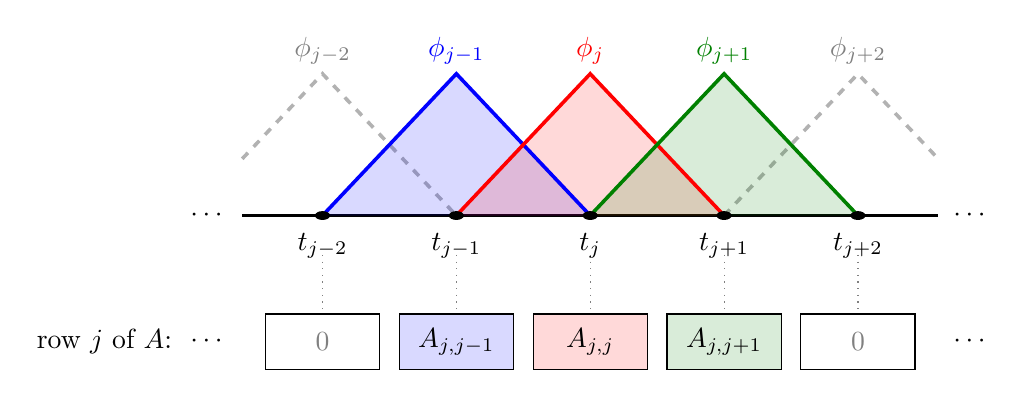
\begin{tikzpicture}[xscale=1.7, yscale=1.0,
    hat/.style={line width=1.3pt},
    entry/.style={draw, minimum width=1.45cm, minimum height=0.7cm, inner sep=1pt},
    ]
    \def\h{1.8}
    \colorlet{cL}{blue}
    \colorlet{cC}{red}
    \colorlet{cR}{green!50!black}
    % grid
    \draw[thick] (0.4,0) -- (5.6,0);
    \node at (0.15,0) {$\cdots$};
    \node at (5.85,0) {$\cdots$};
    % neighbouring hats (no overlap with phi_j)
    \draw[hat, gray!60, dashed] (0.4,0.4*\h) -- (1,\h) -- (2,0);
    \draw[hat, gray!60, dashed] (4,0) -- (5,\h) -- (5.6,0.4*\h);
    % filled hats: overlaps blend
    \fill[cL, opacity=0.15] (1,0) -- (2,\h) -- (3,0) -- cycle;
    \fill[cC, opacity=0.15] (2,0) -- (3,\h) -- (4,0) -- cycle;
    \fill[cR, opacity=0.15] (3,0) -- (4,\h) -- (5,0) -- cycle;
    \draw[hat, cL] (1,0) -- (2,\h) -- (3,0);
    \draw[hat, cC] (2,0) -- (3,\h) -- (4,0);
    \draw[hat, cR] (3,0) -- (4,\h) -- (5,0);
    \node[cL, above] at (2,\h) {$\phi_{j-1}$};
    \node[cC, above] at (3,\h) {$\phi_{j}$};
    \node[cR, above] at (4,\h) {$\phi_{j+1}$};
    \node[gray, above] at (1,\h) {$\phi_{j-2}$};
    \node[gray, above] at (5,\h) {$\phi_{j+2}$};
    % grid points and labels
    \foreach \x/\lab in {1/{t_{j-2}}, 2/{t_{j-1}}, 3/{t_j}, 4/{t_{j+1}}, 5/{t_{j+2}}} {
        \fill[black] (\x,0) circle (1.6pt);
        \node[below=3pt] at (\x,0) {$\lab$};
    }
    % row j of A, columns aligned with the nodes
    \def\yr{-1.6}
    \foreach \x in {1,2,3,4,5} {
        \draw[dotted, gray] (\x,-0.5) -- (\x,\yr+0.35);
    }
    \node[entry, text=gray] at (1,\yr) {$0$};
    \node[entry, fill=cL!15] at (2,\yr) {$A_{j,j-1}$};
    \node[entry, fill=cC!15] at (3,\yr) {$A_{j,j}$};
    \node[entry, fill=cR!15] at (4,\yr) {$A_{j,j+1}$};
    \node[entry, text=gray] at (5,\yr) {$0$};
    \node at (0.15,\yr) {$\cdots$};
    \node at (5.85,\yr) {$\cdots$};
    \node[left] at (-0.05,\yr) {row $j$ of $A$:};
\end{tikzpicture}
\end{document}
